\documentclass[12pt, twoside]{book}
%\documentclass[12pt, oneside]{book}  % single-sided printing

% correct margin setting
\usepackage[a4paper,top=2.5cm,bottom=2.5cm,left=3.5cm,right=2cm]{geometry}
% enabling fonts for UTF8 encoding
\usepackage[utf8]{inputenc}
\usepackage[T1]{fontenc}

% setting line spacing according to the directive
\linespread{1.25} % a value of 1.25 should correspond to 1.5 line spacing

% tells LaTeX not to stretch vertical space to fill the page
\raggedbottom

\usepackage{footnote}

\usepackage{setspace}

\usepackage{tocloft}

\setcounter{tocdepth}{3}    % Controls depth of entries in Table of Contents
\setcounter{secnumdepth}{3} % Controls depth of numbering for section titles


% package for better display of references
\usepackage[backend=biber]{biblatex}
\addbibresource{references.bib}

% package for advanced color usage
\usepackage{xcolor}

\definecolor{background}{rgb}{0.95,0.95,0.95}
\definecolor{placeholder}{rgb}{0.07,0.04,0.56}
\definecolor{string}{rgb}{0.0,0.5,0.0}
\definecolor{highlight}{rgb}{0.8,0.0,0.0}
\definecolor{comment}{rgb}{0.66, 0.66, 0.66}

% package for inserting images
\usepackage{graphicx}

% package for inserting entire pdf documents (thesis assignment)
\usepackage{pdfpages}

% package for properly formatting URLs
\usepackage{url}
% package for hyperlinks within the document (we will remove the colored frames around the lines so that the pdf looks the same as the printed version)
\usepackage[hidelinks,breaklinks]{hyperref}

% package for importing source code
\usepackage{listings}
\usepackage{listings-golang}

\usepackage{cleveref}
\crefname{table}{list}{lists}

\usepackage{tikz}

% package for adjustwidth environment
\usepackage{changepage}

% idk
\usepackage{fancyvrb}

\usepackage{caption}

% package for proper functioning of the figure [H] environment
\usepackage{float}

% package for large tables
\usepackage{longtable}


\setlength{\parindent}{0pt}
\setlength{\parskip}{6pt}

% ---------- CUSTOM COMMAND DEFINITIONS ----------

\makeatletter

% Define new lists with safer file extensions
\newcommand{\listofcommands}{
  {\normalfont\Huge\bfseries List of Commands\par}
  \vspace{2em}
  \@starttoc{cmdlist}
}
\newcommand{\l@cmdlist}{\@dottedtocline{1}{1.5em}{3.5em}}

\newcommand{\listofcodes}{
  {\normalfont\Huge\bfseries List of Codes\par}
  \vspace{2em}
  \@starttoc{codelist}
}
\newcommand{\l@codelist}{\@dottedtocline{1}{1.5em}{3.5em}}

% Add entries to custom lists
\newcommand{\addcommandtolist}[2]{%
  \addcontentsline{cmdlist}{section}{\protect\numberline{#1}#2}
}
\newcommand{\addcodetolist}[2]{%
  \addcontentsline{codelist}{section}{\protect\numberline{#1}#2}
}

\makeatother


\newcommand{\TODO}[1]{\textcolor{blue}{TODO -- #1}}

\newcommand{\shell}{\textcolor{placeholder}{\texttt{$\langle$SHELL$\rangle$}}}
\newcommand{\host}{\textcolor{placeholder}{\texttt{$\langle$HOST$\rangle$}}}
\newcommand{\port}{\textcolor{placeholder}{\texttt{$\langle$PORT$\rangle$}}}
\newcommand{\portt}{\textcolor{placeholder}{\texttt{$\langle$PORT2$\rangle$}}}
\newcommand{\tmp}{\textcolor{placeholder}{\texttt{$\langle$TMP$\rangle$}}}
\newcommand{\script}{\textcolor{placeholder}{\texttt{$\langle$compressed-script$\rangle$}}}
\newcommand{\scriptfile}{\textcolor{placeholder}{\texttt{$\langle$script-filename$\rangle$}}}
\newcommand{\codefile}{\textcolor{placeholder}{\texttt{$\langle$code-filename$\rangle$}}}
\newcommand{\fd}{\textcolor{placeholder}{\texttt{$\langle$fd$\rangle$}}}
\newcommand{\pid}{\textcolor{placeholder}{\texttt{$\langle$pid$\rangle$}}}

\newcommand{\commandpath}[1]{commands/#1}
\newcommand{\imagepath}[1]{images/#1}

\newcommand{\dpd}[1]{\begin{adjustwidth}{10pt}{0pt}\small \textbf{Dependencies:} #1 \end{adjustwidth}}
\newcommand{\notte}[1]{\begin{adjustwidth}{10pt}{0pt} \small \textbf{Note:} #1 \end{adjustwidth}}
\newcommand{\version}[1]{\textbf{Version:} #1}

\newcommand{\inlinecmdline}[1]{\colorbox{background}{\texttt{#1}}}

\newcommand{\lstsettings}[4]
{\lstset{
	language={#1},
	otherkeywords={#3},
	morekeywords=[1]{#3},
	morekeywords=[2]{#4},
	basicstyle={\linespread{0.9}\footnotesize\ttfamily},
	backgroundcolor={\color{background}},
	commentstyle={\color{comment}},
	stringstyle={\color{string}},
	keywordstyle={\color{highlight}},
	keywordstyle=[2]{\color{blue}},
	showspaces=false,
	showstringspaces=false,
	columns=fullflexible,
	breaklines=true,
	escapechar={#2},
	frame=single,
	rulecolor={\color{black}},
	framesep=5pt,
	framerule=0.8pt
}}

\newenvironment{cmdline}[3]
{\begingroup
\lstsettings{bash}{#1}{#2}{#3}
\VerbatimOut{tmp.txt}}
{\endVerbatimOut
\lstinputlisting{tmp.txt}
\endgroup}


\newcounter{cmdctr}[section]
\renewcommand{\thecmdctr}{\thesection.\arabic{cmdctr}}
\crefname{cmdctr}{command}{commands}

\newcommand{\getcmdline}[7]{
\refstepcounter{cmdctr}
\addcommandtolist{\thecmdctr}{#5}
\begin{minipage}{\linewidth}
\lstsettings{bash}{#2}{#3}{#4}
\lstinputlisting[title={Command \thecmdctr: #5}, label={cmd:#6}]{#1}
\end{minipage}
#7}


\newcounter{codectr}[section]
\renewcommand{\thecodectr}{\thesection.\arabic{codectr}}
\crefname{codectr}{code}{codes}

\newcommand{\getcode}[8]{
\refstepcounter{codectr}
\addcodetolist{\thecodectr}{#6}
\begin{minipage}{\linewidth}
\lstsettings{#2}{#3}{#4}{#5}
\lstinputlisting[title={Code \thecodectr: #6}, label={code:#7}]{#1}
\end{minipage}
#8}

% ------------------------------------------------

\def\mfrok{2025}
\def\mfnazov{Analysis of reverse shell techniques and possible countermeasures}
\def\mftyp{Bachelor Thesis}
\def\mfautor{Matúš Bucher}
\def\mfskolitel{Ing. Dušan Bernát, PhD.}

\def\mfmiesto{Bratislava, \mfrok}

\def\mfodbor{Computer Science}
\def\program{Computer Science }

\def\mfpracovisko{ Department of Computer Science }

\begin{document}
\frontmatter
\pagestyle{empty}

% -------------------
% ----- Obalka ------
% -------------------

\begin{center}
  \sc\large
  Comenius University in Bratislava\\
  Faculty of Mathematics, Physics and Informatics

\vfill

{\LARGE\mfnazov}\\
\mftyp
\end{center}

\vfill

{\sc\large 
\noindent \mfrok\\
\mfautor
}

\cleardoublepage
% --- koniec obalky ----

% -------------------
% --- Titulný list
% -------------------

\noindent

\begin{center}
\sc  
\large
  Comenius University in Bratislava\\
  Faculty of Mathematics, Physics and Informatics

\vfill

{\LARGE\mfnazov}\\
\mftyp
\end{center}

\vfill

\noindent
\begin{tabular}{ll}
Study Programme: & \program \\
Field of Study: & \mfodbor \\
Department: & \mfpracovisko \\
Supervisor: & \mfskolitel \\
\end{tabular}

\vfill


\noindent \mfmiesto\\
\mfautor

\cleardoublepage
% --- Koniec titulnej strany


% -------------------
% --- Zadanie z AIS
% -------------------
% v tlačenej verzii s podpismi zainteresovaných osôb.
% v elektronickej verzii sa zverejňuje zadanie bez podpisov
% v pracach v anglictine anglicke aj slovenske zadanie

\newpage
\setcounter{page}{3}
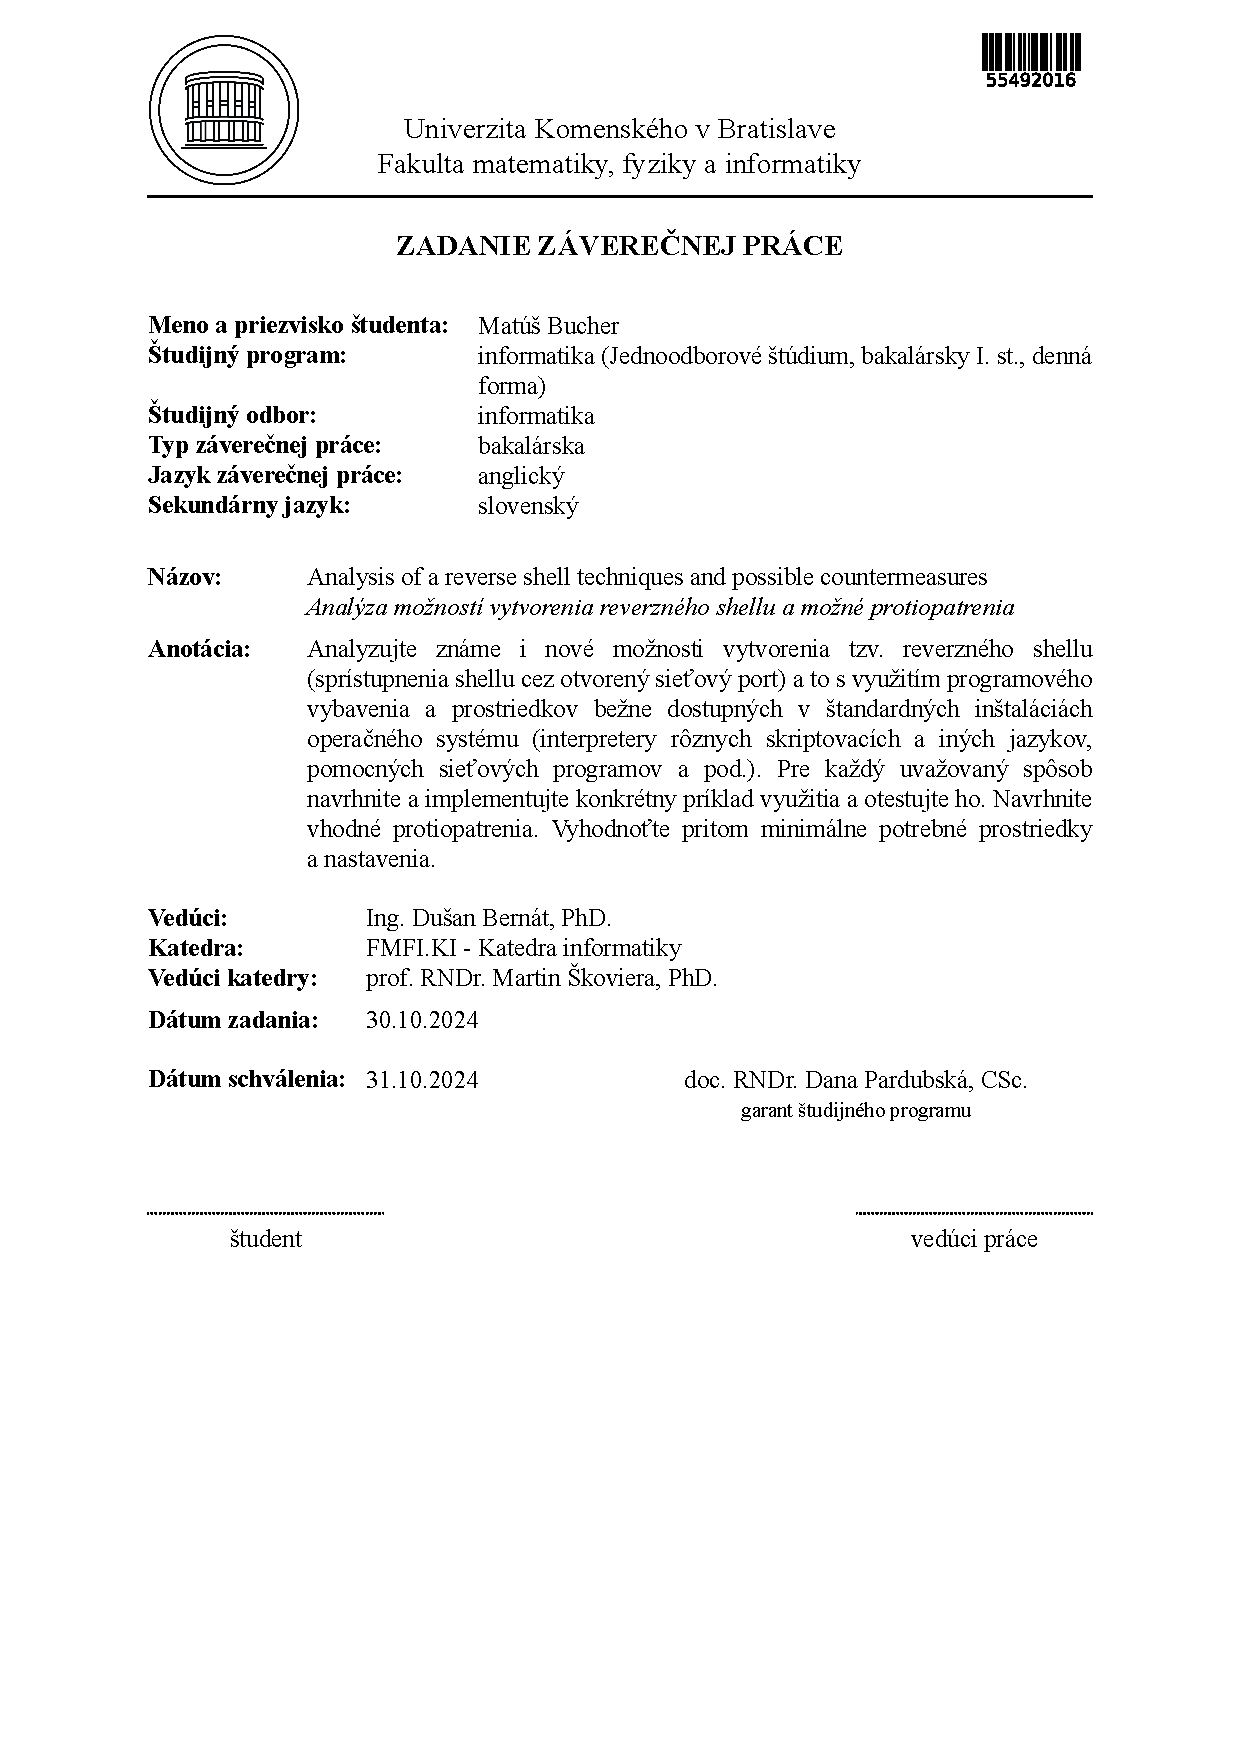
\includepdf{images/zadanie.pdf}


\includepdf{images/zadanie-en.pdf}

% --- Koniec zadania


% -------------------
%   Poďakovanie - nepovinné
% -------------------
\newpage
\pagestyle{plain}
~

\vfill
{\bf Acknowledgments:} I would like to thank my supervisor, Ing.\ Dušan Bernát, PhD.\ for his guidance and advice.

% --- Koniec poďakovania

% -------------------
%   Abstrakt - Slovensky
% -------------------
\newpage
\section*{Abstrakt}

Reverzný shell je bežnou technikou, ktorú útočníci používajú na získanie neoprávneného prístupu k vzdialeným systémom. Táto práca poskytuje komplexnú analýzu metód reverzných shellov, so zameraním na tie, ktoré využívajú nástroje bežne dostupné v štandardných inštaláciách Linuxových systémov. Ponúkame široký zoznam techník zahŕňajúcich sieťové nástroje, shellové interprety, programovacie jazyky a ďalšie systémové nástroje. Každá metóda bola implementovaná a testovaná v kontrolovanom prostredí, aby sa vyhodnotila jej efektívnosť a minimálne závislosti. Okrem vymenovania samotných techník sa práca zaoberá aj protiopatreniami a odporúčaniami na ochranu pred útokmi pomocou reverzných shellov.

Na podporu ďalšieho výskumu a experimentovania sme vytvorili jednoduchý testovací framework založený na Makefile, ktorý automatizuje vykonávanie všetkých analyzovaných metód.

\paragraph*{Kľúčové slová:} reverzný shell, techniky typu living-off-the-land, systémové nástroje, protiopatrenia
% --- Koniec Abstrakt - Slovensky


% -------------------
% --- Abstrakt - Anglicky 
% -------------------
\newpage 
\section*{Abstract}

Reverse shells are a common technique used by attackers to gain unauthorized remote access to systems. This thesis provides a comprehensive analysis of reverse shell methods, focusing on those that utilize tools typically found in standard Linux-based system installations. We list a broad set of techniques involving network utilities, shell interpreters, programming language runtimes, and other system tools. Each method was implemented and tested in a controlled environment to assess its effectiveness and minimal dependencies. Beyond the enumeration of these techniques, the thesis explores countermeasures and best practices for protection against reverse shell attacks.

To facilitate further research and experimentation, we developed an easy-to-use testing framework based on a Makefile, which automates the execution of all analyzed methods.


\paragraph*{Keywords:} reverse shell, living-off-the-land techniques, system utilities, countermeasures

% --- Koniec Abstrakt - Anglicky

% -------------------
% --- Predhovor - v informatike sa zvacsa nepouziva
% -------------------
%\newpage 
%
%
%\chapter*{Preface} %
%
%Predhovor je všeobecná informácia o práci, obsahuje hlavnú charakteristiku práce 
%a okolnosti jej vzniku. Autor zdôvodní výber témy, stručne informuje o cieľoch 
%a význame práce, spomenie domáci a zahraničný kontext, komu je práca určená, 
%použité metódy, stav poznania; autor stručne charakterizuje svoj prístup a svoje
%hľadisko. 
%
% --- Koniec Predhovor


% -------------------
% --- Obsah
% -------------------

\cleardoublepage 

\tableofcontents

% ---  Koniec Obsahu

% -------------------
% --- Zoznamy tabuliek, obrázkov - nepovinne
% -------------------

\newpage 

\listoftables

\newpage 

\listofcommands

\newpage 

\listofcodes

% ---  Koniec Zoznamov

\mainmatter
\pagestyle{headings}

\input intro.tex 

\input chapters/chapter1.tex

\input chapters/chapter2.tex

\input chapters/chapter3.tex

\input chapters/chapter4.tex

\input conclusion.tex



%\input zaver.tex

% -------------------
% --- Bibliografia
% -------------------


\newpage	

\backmatter

\thispagestyle{empty}
\clearpage

\printbibliography 

%---koniec Referencii

% -------------------
%--- Prilohy---
% -------------------

\input appendix-A.tex

\input appendix-B.tex

\end{document}
